\documentclass[fleqn, 11pt, a4paper]{book}

\usepackage{titlesec}
\usepackage[spanish]{babel}
\usepackage{afterpage}
\usepackage{graphicx}
\usepackage{fancyhdr}
\usepackage[left=2.5cm,top=2.5cm,right=2.5cm,bottom=2.5cm]{geometry}
\usepackage{float}
\usepackage{multicol}
\usepackage{array}
\usepackage{amsmath}
\usepackage{amsfonts}
\usepackage[none]{hyphenat}
\usepackage{mathtools}
\usepackage{dsfont}
\usepackage{amssymb}
\usepackage{color, colortbl}
\usepackage{pifont}
\usepackage{bm}
\usepackage{stackengine}
\usepackage{multirow}
\usepackage[table]{xcolor}
\usepackage{xcolor}
\usepackage{hhline}
\usepackage{scalerel}
\usepackage{diagbox}
\usepackage{cancel}
\usepackage[hidelinks]{hyperref}
\usepackage{listings}
\usepackage{pdfpages}
\usepackage{minitoc}
\usepackage{appendix}


%%%%%%%%%%%%%%%%%%%%%%%%%%%%%%%%%%%%%%%%%%%%%%%%%%%
\spanishdecimal{'}



\setlength{\headheight}{1.5cm}
\setlength{\headsep}{1cm}
\setlength{\footskip}{0cm}

\graphicspath{ {images/} }
\renewcommand\labelenumii{\theenumi.\arabic{enumii}.}
\renewcommand{\chaptername}{}

\newcommand\blankpage{%
  \null
  \thispagestyle{empty}%
  \newpage}

\pagestyle{fancy}
\fancyhf{}
\fancyhead[L]{{\scshape\large LogicUS: La Lógica Proposicional y la Lógica de Primer Orden bajo el paradigma funcional y la orientación Web.}\\ {\normalfont Autor : \textit{Ramos González, Víctor.}}}
\fancyfoot[C]{ \leftmark }
\fancyfoot[R]{ \thepage }

% Abstract estilo

\newenvironment{abstract}{%
\thispagestyle{empty}
\begin{minipage}{\textwidth}
\setlength{\parskip}{0.5cm}
\setlength{\parindent}{1.5cm}
\noindent\rule{\textwidth}{1pt}

\vspace{0.2cm}

\noindent{\LARGE \textsc{Resumen}}\\
\noindent\rule{\textwidth}{1pt} 

\vspace{1cm}

}
{\end{minipage}
\newpage}

\newenvironment{acknowledgments}{%
\thispagestyle{empty}
\begin{minipage}{\textwidth}
\setlength{\parskip}{0.5cm}
\setlength{\parindent}{1.5cm}
\noindent\rule{\textwidth}{1pt}

\vspace{0.2cm}

\noindent{\LARGE \textsc{Agradecimientos}}\\
\noindent\rule{\textwidth}{1pt} 

\vspace{1cm}

}
{\end{minipage}
\newpage}

%=======================================
\includeonly
{
	sections/portada,
	sections/resumen,
	sections/agradecimientos,
	sections/cap1,
}

\sloppy
\begin{document}

\setlength{\parskip}{0.5cm}

\renewcommand{\listtablename}{Índice de tablas}
\renewcommand{\tablename}{Tabla}

\renewcommand{\lstlistlistingname}{Índice de fragmentos de código}
\renewcommand{\lstlistingname}{Código}
\renewcommand{\mtctitle}{}

\dominitoc

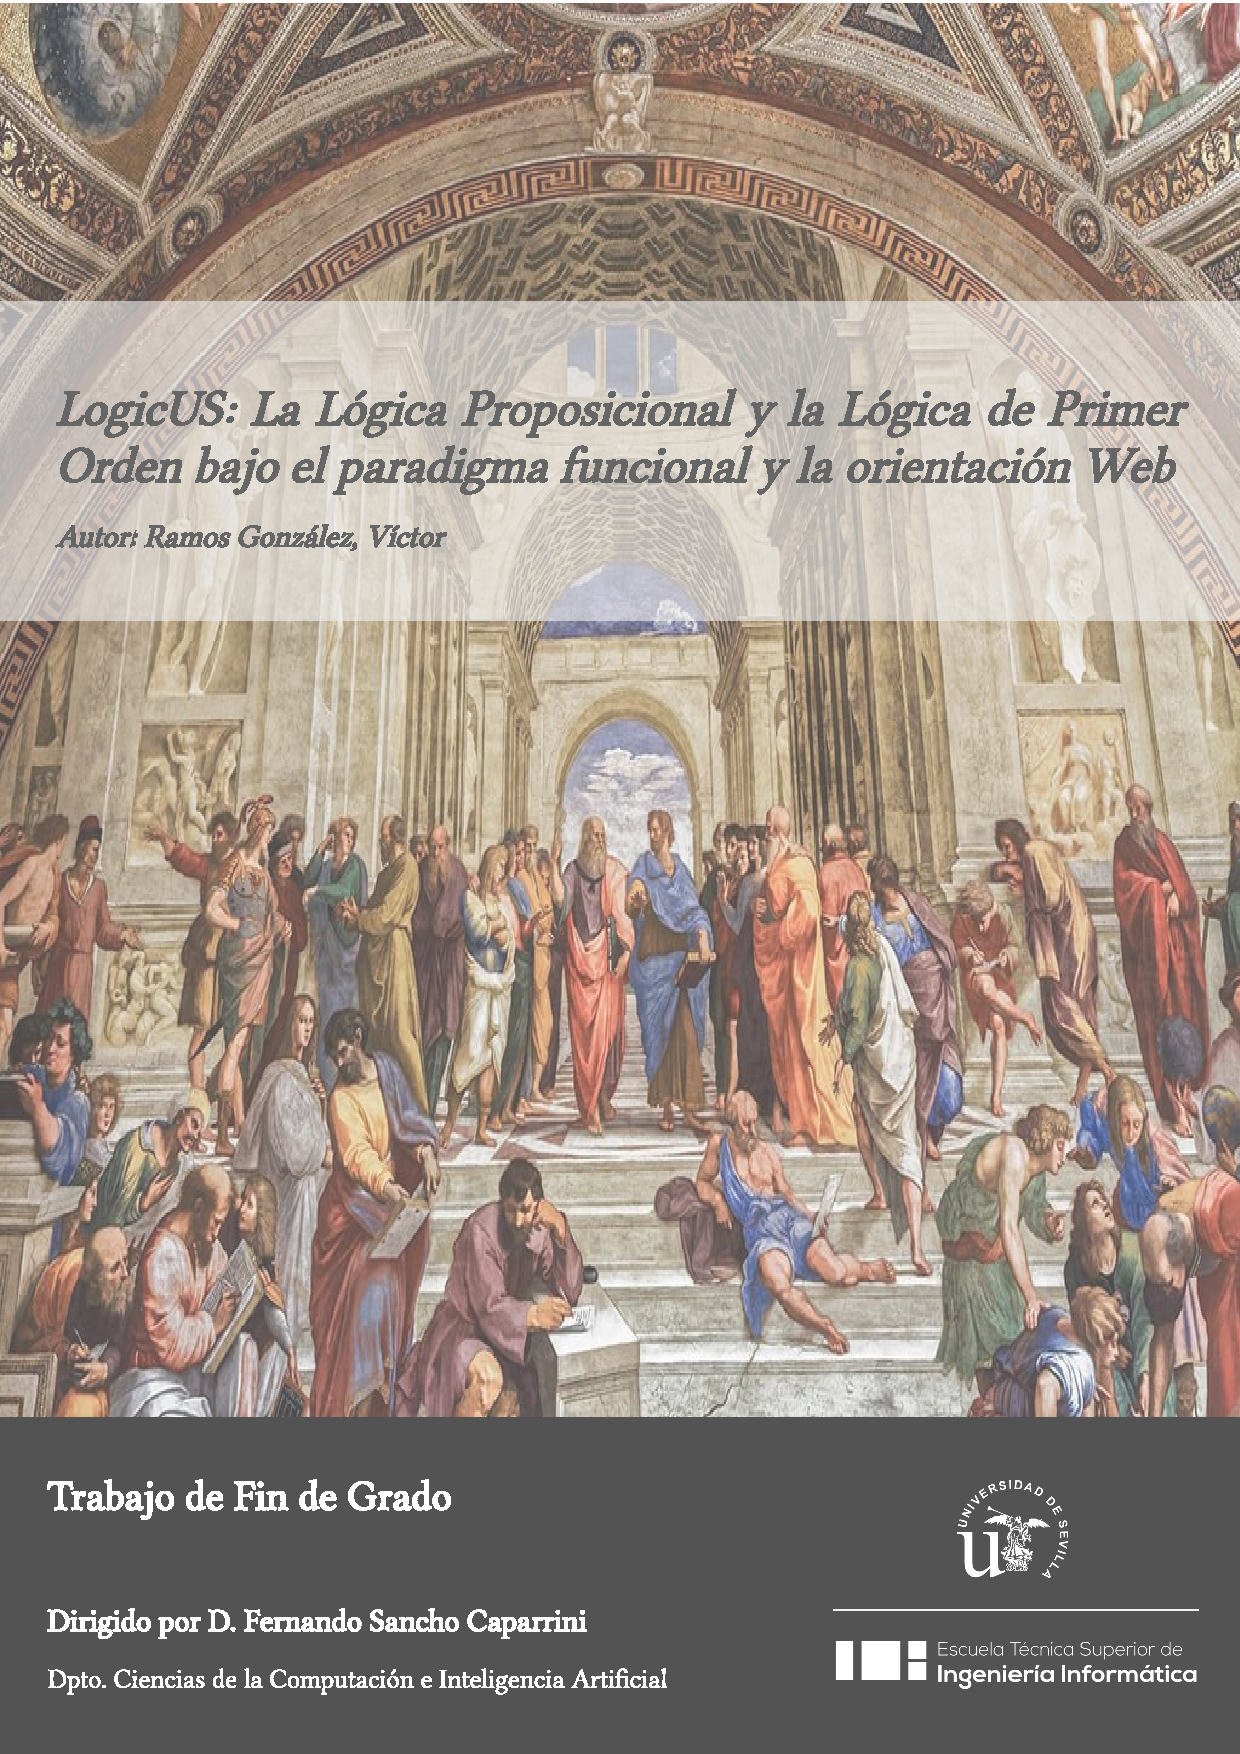
\includepdf[scale=1]{sections/portada.pdf}

\blankpage

\begin{titlepage}
\begin{center}

\includegraphics[scale=0.12]{logoETSIIUS.png}

\vspace{1cm}

{\large \textsc{Universidad de Sevilla \\ Escuela Técnica Superior de Ingeniería Informática.}}

\vspace{0.5cm}

{\large \textsc{G.I.I. Tecnologías Informáticas.}}

\vspace{1cm}

{\Large \textsc{Trabajo de Fin de Grado}}

\vspace{1cm}


{\LARGE LogicUS: La Lógica Proposicional y la Lógica de Primer Orden bajo el paradigma funcional y la orientación Web.}

\vspace{1cm}

{\large \textsc{Realizado por:}}

{\large Ramos González, Víctor}

\vspace{1cm}

{\large \textsc{Dirigido por:}}

{\large D. Fernando Sancho Caparrini}

\vspace{1cm}

{\large \textsc{Departamento}}

{\large Ciencias de la Computación e Inteligencia Artificial.}
\end{center}

\vspace{1cm}
\begin{flushright}
\textit{Sevilla a ... de ... del 2021 \quad}
\end{flushright}
\end{titlepage}


\blankpage

\begin{abstract}

El proyecto realiza un estudio de las distintas herramientas existentes para el trabajo con la Lógica Proposicional y la Lógica de Primer Orden, de forma que aborden de una forma clara, sencilla y visual muchos de los principales algoritmos para el tratamiento de dichas lógicas.

En estos términos, y ante la imposibilidad de encontrar una que cubra los requisitos expuestos, este proyecto pretende aportar una herramienta para el tratamiento de la Lógica Computacional en un ámbito académico,  posibilitando el trabajo con conjuntos de fórmulas de proposicionales y de lenguajes de primer orden (incluyendo lenguajes con igualdad), con el desarrollo de distintos algoritmos bajo el paradigma de la programación declarativa, de manera que proporcione una herramienta capaz de servir como apoyo docente tanto al profesorado como al alumnado, y a estos efectos aglutina en sus distintos componentes y modalidades la capacidad de trabajo desde un enfoque más cercano al paradigma declarativo y la notación funcional al mismo tiempo que, a través del manejo de la interfaz web, proporciona la capacidad de un uso completo y sencillo de las funcionalidades provistas.

El proyecto se centra principalmente en el desarrollo de módulos del lenguaje Elm, que permite además el trabajo multiplataforma, a través del uso de la propia consola (\textit{elm-repl}), o a través de la compilación de los propios módulos al lenguaje web \textit{javascript}, permitiendo la integración con sistemas para la creación de documentos \textit{.html} y \textit{.md} (integración con \textit{gicentre/litvis}) o el desarrollo de una interfaz web, marcada por la accesibilidad y la usabilidad.
\end{abstract}

\blankpage


\begin{acknowledgments}



\end{acknowledgments}

\blankpage

\setcounter{page}{1}%

\renewcommand{\contentsname}{Índice de contenidos}

\pagestyle{empty}
\tableofcontents

\addtocontents{toc}{\textbf{Contenidos}\hfill \textbf{Página} \par}
\addtocontents{toc}{\vspace{-2mm} \hspace{-7.5mm} \hrule \par}

%\newpage
%\listoftables

%\newpage
%\lstlistoflistings

\newpage

\pagestyle{fancy}


\chapter{Introducción.}
\minitoc

\newpage
\section{Visión general del capítulo}

\section{Marco de desarrollo del proyecto.}

\subsection{Motivación del proyecto.}

\subsection{Contexto del proyecto.}

\subsection{Objetivos.}

\section{Metodología de desarrollo del proyecto.}

\subsection{Objetivos específicos y herramientas utilizadas.}

\subsection{Planificación y organización del proyecto.}




\chapter{El lenguaje Elm.}

\minitoc

\newpage

\section{Visión general del capítulo}
\section{Introducción a la Programación Declarativa.}
\section{Elm como herramienta de Programación Declarativa.}
\section{Elm como herramienta orientada a la Web.}


\chapter{Desarrollo del núcleo de LogicUS}

\minitoc

\newpage

\section{Visión general del capítulo}

\section{Trabajo con la Lógica Proposicional}
\subsection{Módulos \textit{SintaxSemanticsPL} y \textit{SintaxSemanticsPL.IO}}
\subsection{Módulos \textit{SemanticBoardsPL} y \textit{SemanticBoardsLP.IO}}
\subsection{Módulos \textit{NormalFormsClausesPL} y \textit{NormalFormsClausesPL.IO}}
\subsection{Módulos \textit{DPLL} y \textit{DPLL.IO}}
\subsection{Módulos \textit{DeductiveSystemsPL} y \textit{DeductiveSystemsPL.IO}}
\subsection{Módulos \textit{ResolutionPL} y \textit{ResolutionPL.IO}}

\section{Trabajo con la Lógica de Primer Orden}
\subsection{Módulos \textit{SintaxSemanticsFOL} y \textit{SintaxSemanticsFOL.IO}}
\subsection{Módulos \textit{SemanticBoardsFOL} y \textit{SemanticBoardsFOL.IO}}
\subsection{Módulos \textit{NormalFormsClausesFOL} y \textit{NormalFormsClausesFOL.IO}}
\subsection{Módulos \textit{Herbrand} y \textit{Herbrand.IO}}
\subsection{Módulos \textit{UnificationFOL} y \textit{UnificationFOL.IO}}
\subsection{Módulos \textit{ResolutionFOL} y \textit{ResolutionFOL.IO}}



\chapter{Desarrollo de la interfaz de LogicUS}

\minitoc

\newpage

\section{Visión general del capítulo}

\section{Trabajo con la Lógica Proposicional}

\section{Trabajo con la Lógica de Primer Orden}

\chapter{Trabajo con Lógicus}

\minitoc

\newpage

\section{Trabajo con la shell de Elm.}
\section{Creación de documentos web. Integración con el proyecto \textit{gicentre/litvis}}
\section{Acceso y manejo de la interfaz web.}

\chapter{Conclusiones}

\minitoc

\newpage
\section{Visión general del capítulo}


\appendix
\addcontentsline{toc}{chapter}{Apéndices}

\chapter{Implementación de los módulos de la Lógica Proposicional.}

\minitoc

\section{Visión general del apéndice}
\section{Implementación del módulo SintaxSemanticsPL}
\section{Implementación del módulo SintaxSemanticsPL.IO}
\section{Implementación del módulo SemanticBoardsPL}
\section{Implementación del módulo SemanticBoardsPL.IO}
\section{Implementación del módulo NormalFormsClausesPL}
\section{Implementación del módulo NormalFormsClausesPL.IO}
\section{Implementación del módulo DPLL}
\section{Implementación del módulo DPLL.IO}
\section{Implementación del módulo DeductiveSystemsPL}
\section{Implementación del módulo DeductiveSystemsPL.IO}
\section{Implementación del módulo ResolutionPL}
\section{Implementación del módulo ResolutionPL.IO}

\chapter{Implementación de los módulos de la Lógica de Primer Orden.}

\minitoc

\section{Visión general del apéndice}
\section{Implementación del módulo SintaxSemanticsFOL}
\section{Implementación del módulo SintaxSemanticsFOL.IO}
\section{Implementación del módulo SemanticBoardsFOL}
\section{Implementación del módulo SemanticBoardsFOL.IO}
\section{Implementación del módulo NormalFormsClausesFOL}
\section{Implementación del módulo NormalFormsClausesFOL.IO}
\section{Implementación del módulo Herbrand}
\section{Implementación del módulo Herbrand.IO}
\section{Implementación del módulo UnificationFOL}
\section{Implementación del módulo UnificationFOL.IO}
\section{Implementación del módulo ResolutionFOL}
\section{Implementación del módulo ResolutionFOL.IO}

\chapter{Implementación de la Interfaz}
\section{Visión general del apéndice}
\section{...}




\end{document}






